\documentclass{article}
\usepackage{graphicx}
\usepackage[margin=1.5cm]{geometry}
\usepackage{amsmath}

\begin{document}

\title{Tuesday Reading Assessment: Chapter 6}
\author{Prof. Jordan C. Hanson}

\maketitle

\section{Functions of Combinatorial Logic: Adders/Subtractors, Comparators, and Decoders/Encoders}

\begin{figure}[ht]
\centering
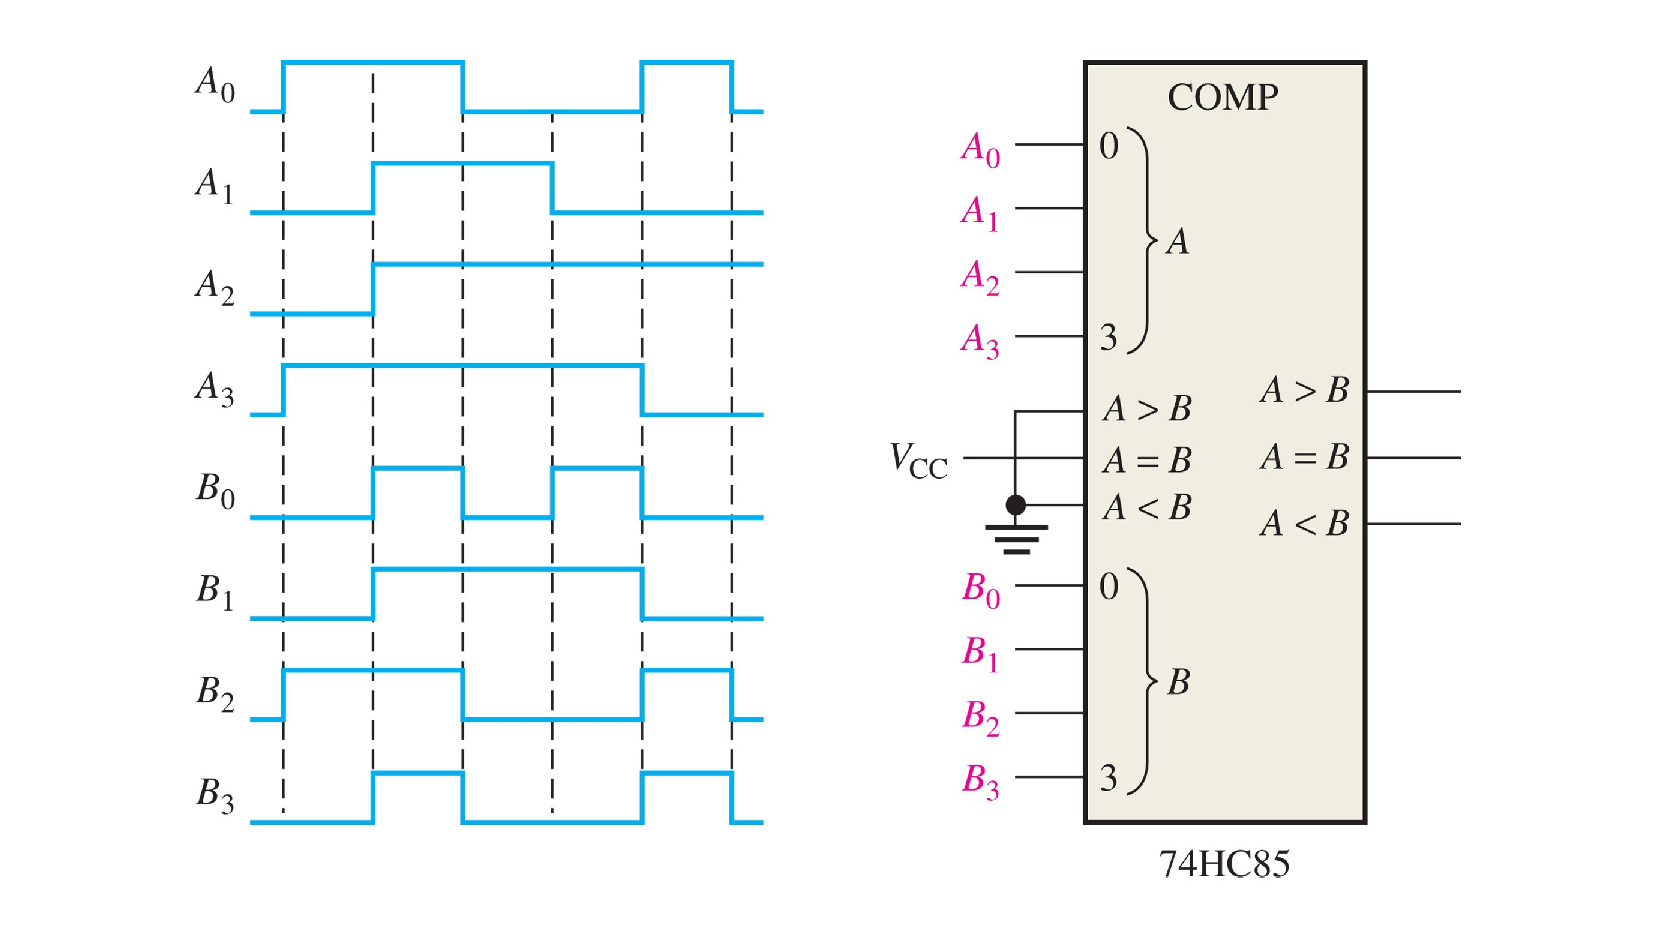
\includegraphics[width=0.4\textwidth,trim=2cm 0cm 2cm 0cm,clip=true]{figures/quiz2.pdf}
\caption{\label{fig:quiz1} A logic circuit collecting two 4-bit binary numbers, with (effectively) one output.}
\end{figure}

\begin{enumerate}
\item Given the input timing diagram in Fig. \ref{fig:quiz1}, what is the output waveform of the logic circuit? \\ \vspace{1cm}
\item Figure \ref{fig:quiz2} resembles a 4-bit FA (full adder).  (a) The middle row of gates are XNOR gates.  Show that B XNOR HIGH equals B, and that B XNOR LOW equals NOT B.  (b) Taking A and B data from the first time bin in Fig. \ref{fig:quiz1} (left), compute the $\Sigma$ outputs if $\bar{Add}/Subt$ is HIGH. (c) What would the outputs be if $\bar{Add}/Subt$ is LOW?
\end{enumerate}

\begin{figure}[hb]
\centering
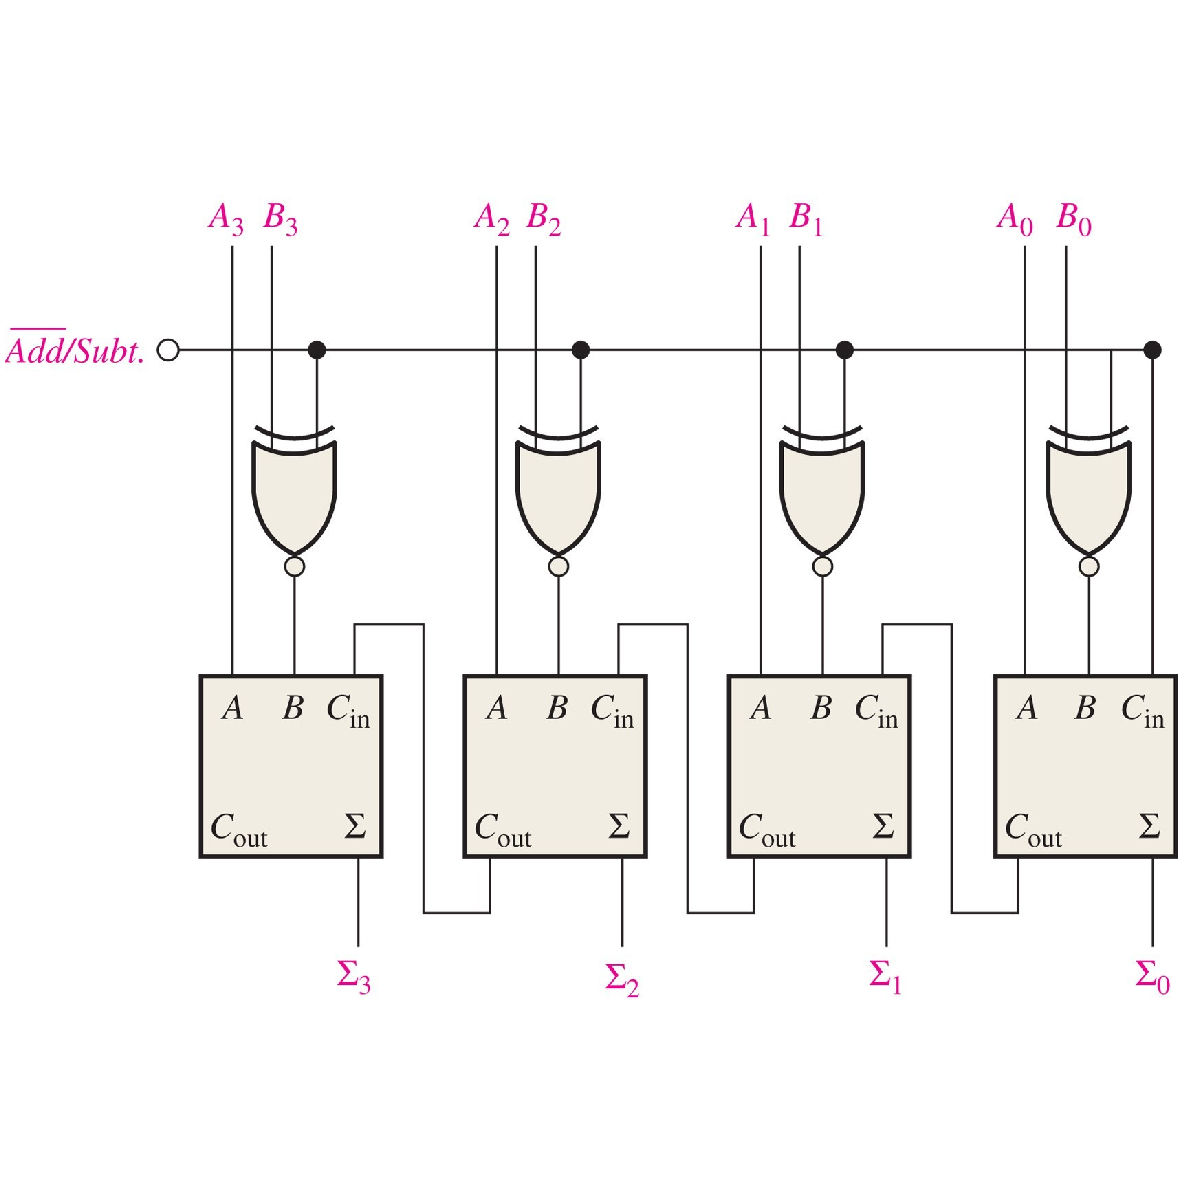
\includegraphics[width=0.45\textwidth,trim=0cm 2cm 0cm 2cm,clip=true]{figures/quiz1.pdf}
\caption{\label{fig:quiz2} A 4-bit FA with an additional feature.}
\end{figure}

\end{document}
